\providecommand{\main}{../../main}
\documentclass[../../main/main.tex]{subfiles}


\begin{document}

% \section{Numerical simulation of the experiment}

% To simulate the angular distribution of the particles we wrote a Python package with two main objectives: in first place the simulation will allow us to plan the acquisitions, moreover the simulated distributions will provide us a theoretical reference to  compare with our experimental result. This last usage is of particular importance since the $\sim\frac{1}{\sin^4 (\theta /2)}$ expected behaviour does not take into account the geometry of the experiment which, especially for the ALPIDE detector, has a significant impact on the final distribution.



% \subsection{Beam simulation}

% Inside the Python package we built a series of objects, each one representing a particular piece of our setup. The system of reference of choice has origin at center of the vacuum chamber, the z-axis along the beam line and the y-axis pointing upward. In order to run the simulation the positions of all the setup component have been measured in this system as shown in \tabref{tab:dist}. In the following a brief remind of the most important positions is reported:
% \begin{itemize}
%     \item $\bar{z}_{source} = 21$mm : radioactive source distance from target
%     \item $\bar{z}_{C1} = 19.5$mm and $\bar{z}_{C2} = 1$mm : distance of the two collimators
%     \item $\bar{d}_{Si}=92$mm $\bar{d}_{A}=78.6$ mm distance of the detectors from target
% \end{itemize}

% The generation and evolution of the particle is then computed through a Monte Carlo simulation procedure, whose steps are described in the following.

% \paragraph{Particle generation} Given the position of the source and its radius $r_s = 0.335$ a specified number of particles are generated with energy taken from the dsitribution shown is \figref{fig:alphasim}. To each particle is associated a position $\bar{x}_i$, uniformly generated inside a circumference of radius $r_s$ around the source, and a momentum, randomly generated in the forward hemisphere, obtaining a good simulation of our source.


% \paragraph{Beam collimation} After the generation each particle evolution is analytically computed until its position along the z-axis is equal to the one of the first collimator. At this point the collimation is simulated. Naming with $w$ and $h$ respectively the height and width of the collimator the following conditions are imposed: 
% $$|x_i - x_{C1}| \leq w/2 \qquad
% |y_i - y_{C1}| \leq h/2 $$

% All those particles not satisfying both the considtions are discarded. The same procedure is then applied a second time to simulate the passage through the second collimator.

% \paragraph{Target scattering}
% The interaction with the gold foil is composed of the following passages:
% \begin{itemize}
%     \item For each particle an impact parameter $b$ is randomly generated between $0$     and the mean inter-atomic distance between the gold atoms
%     \item The scattering angles are computed. The azimuthal angle is randomly     generated, $\alpha\in [0,2\pi]$ while the polar angle is computed from the impact parameters as:
%     $$
% \theta=\pi-2 \cos ^{-1} \frac{k / 2 E_{\alpha} b}{\sqrt{1+\left(k^{2} /\left(2 E_{\alpha} b\right)^{2}\right)}} \quad \text{with} \quad
% k=q_\alpha Z / 4 \pi \varepsilon_{0}
% $$
%  where $E_\alpha$ is the enrgy of the particle, $q_\alpha$ its charge and $Z$ the atomic number of the target.

%     \item Each particle momenta is rotated using the rotation matrices generated from the scattering angles.
% \end{itemize}

% During the computations the following corrections are also considered in order to obtain a better simulation of the physical process:
%     \begin{itemize}
%         \item Shielded charge: the effective charge depends on the impact parameter, the exact value is computed using an exponential interpolation
%         \item Energy loss due to interaction: each particle momenta is reduced taking into account the energy loss caused by the passage through the foil
%     \end{itemize}
    
% \paragraph{Detector acquisition}
% Similarly to what done for the collimator the detection of the scattered particles is computed making them evolve until reaching a distance from the center equal to the detectors one. For the ALPIDE detection the particles are required to satisfy 
% $ |y_i - y_{C1}| \leq h/2 $;
% while, for the silicon detector, $ |y_i - y_{C1}| \leq r_p/2 $ is imposed.

% \paragraph{Angular distribution} The particles that have not been discarded are the ones detected, from their position we compute the angular distribution, always taking the center of the vacuum chamber as reference. 

% \subsection{Validation through beam profile}

% In order to validate the simulation package and procedure we simulated the beam profile of the radioactive source. This simulation can be run by just imposing a null charge and thickness target. In this way we are effectively simulating a situation where the target foil has not been inserted. In \figref{fig:profile} the comparison between the simulated data and the experimental curve for both detectors is shown. As we can see the two curves have a very high agreement, validating out simulation procedure.

% \begin{figure*}[h]
%     \begin{minipage}[c]{0.49\linewidth}
%         \vspace{0pt}
%         \centering
%         \subfloat[SSB detector beam profile]{
%             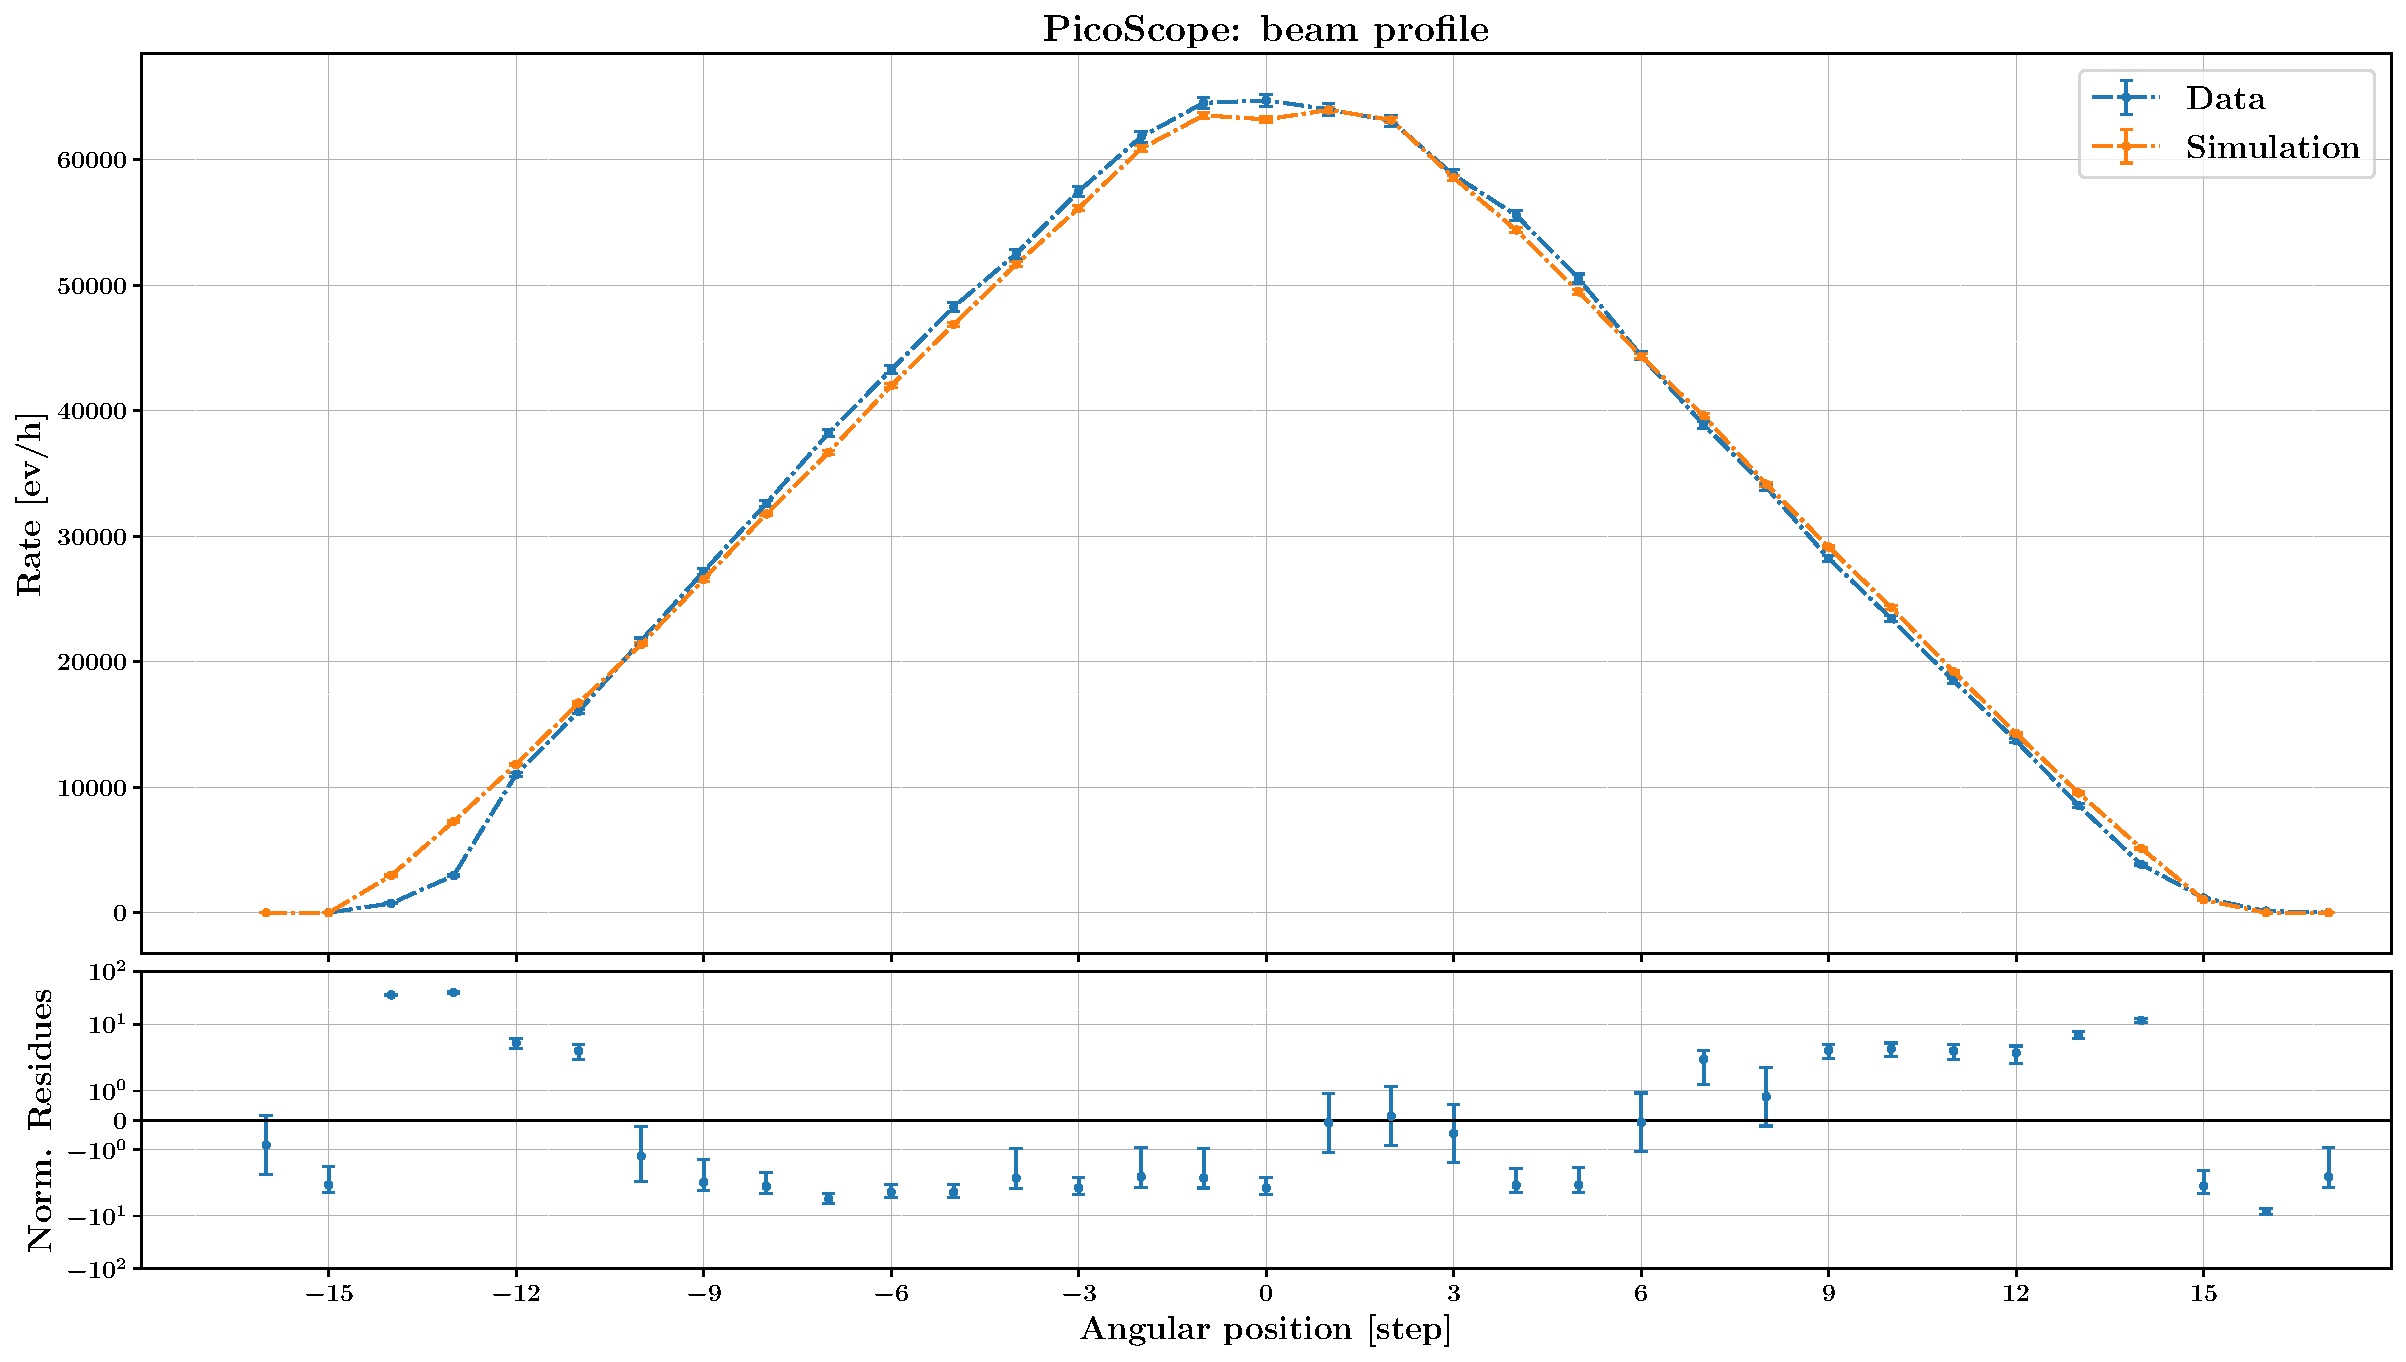
\includegraphics[width=\textwidth]{../sections/04/images/picoscope/beam_profile.pdf}
%     % \caption{Beam profile acquired with the ALPIDE detector. Comparison between simulation and experimental curve}
%             \label{fig:profile_picoscope}
%         }
%     \end{minipage}
%     \hfill
%     \begin{minipage}[c]{0.49\linewidth}
%         \vspace{0pt}
%         \centering
%         \subfloat[ALPIDE detector beam profile]{
%             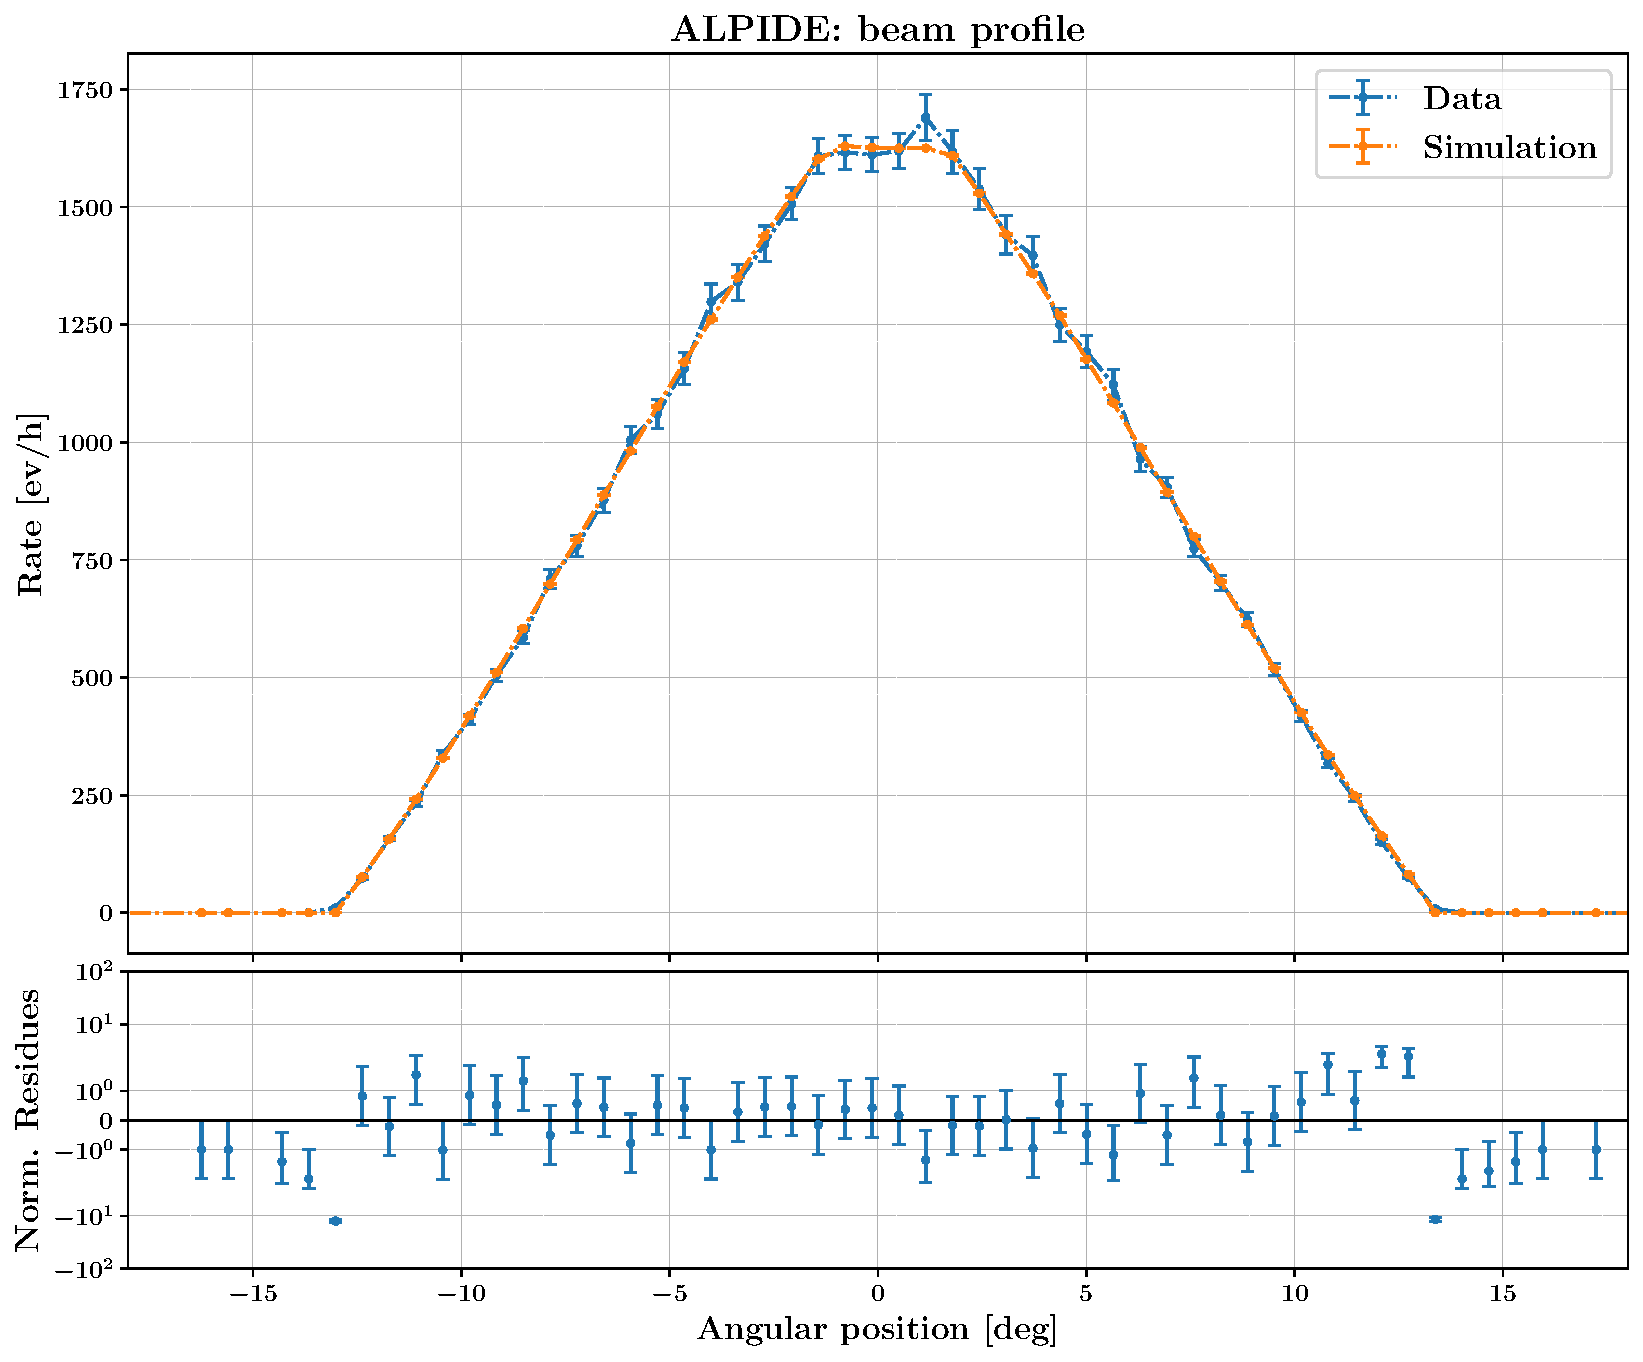
\includegraphics[width=\textwidth]{../sections/04/images/ALPIDE/ALPIDE_beam_profile.pdf}
%     % \caption{Beam profile acquired with the ALPIDE detector. Comparison between simulation and experimental curve}
%             \label{fig:profile_ALPIDE}
%         }
%         % \caption{Beam profile acquired with the silicon detector. Comparison between simulation and experimental curve}   
%     \end{minipage}
%     \label{fig:profile}
%     \caption{Beam profile comparison between the numerical simulation and the acquired spectrum with the ALPIDE detector in \figref{fig:profile_ALPIDE} and the SSB detector \figref{fig:profile_picoscope}.}
% \end{figure*}

\end{document}
